\documentclass[12pt,a4paper]{article}
\usepackage{graphicx}
\usepackage{amsmath}
\usepackage{amssymb}
\usepackage[colorlinks=true, allcolors=blue]{hyperref}
\usepackage{url}
\usepackage[style=apa, backend=biber]{biblatex}
\usepackage[german]{babel}

\usepackage{helvet}
\renewcommand{\familydefault}{\sfdefault}

\usepackage[left=3cm,top=3cm,right=3cm,bottom=3cm,bindingoffset=0.5cm]{geometry}
\renewcommand{\baselinestretch}{1.5} 

\addbibresource{references.bib}

\title{Musterlösung Kurvendiskussion einer Funktionsschar}
\author{Danilo Stojanovic, Tim Gabrikowski}
\date{\today}

\begin{document}

\maketitle

\begin{abstract}
In diesem Dokument wird eine Kurvendiskussion an einer Funktionsschar durchgeführt. Eine Funktionsschar ist eine Menge von Funktionen, die durch einen gemeinsamen Parameter oder mehrere Parameter beschrieben werden. Diese Parameter können unterschiedliche Werte annehmen, wodurch verschiedene Funktionen innerhalb der Schar entstehen.
\end{abstract}

\newpage

\section{Funktionsschar}

Die zu Analysierende Funktionsschar ist die Folgende:

\begin{equation}
    \label{eq:function}
    \begin{aligned}
        f_k(x)&=(x-k)^2+\frac{k}{2} \\ 
        &= x^2 - 2kx + k^2 + \frac{k}{2}
    \end{aligned}
\end{equation}

\section{Kurvendiskussion}

\subsection{Definitionsbereich}

Es handelt sich bei der Funktionsschar um eine ganzrationale Funktion 2. Grades, also ist der Definitionsbereich der Zahlenraum der reelen Zahlen.

\begin{equation}
    \label{eq:defB}
    D_{f_k} = \mathbb{R}
\end{equation}

\subsection{Grenzverhalten}

Da es sich um eine Funktion 2. Grades, also graden Grades handelt kommt diese aus dem unendlichen und verläuft in die gleiche Richtung ins unendliche. Vor dem $x^2$ steht ein positiver Faktor ($1$), also kommt die Funktion aus dem positiv unendlichen und verläuft ins positiv unendliche.

\begin{equation}
    \label{eq:lim}
    \lim_{x \to \pm \infty} f(x) = + \infty
\end{equation}

\subsection{Achsenschnittpunkte}

\subsubsection{Y-Achsenschnittpunkt}

Den Schnittpunkt mit der Y-Achse berechnet man, indem man $x=0$ in die Funktionsschar einsetzt. 

\begin{equation}
    \label{eq:spyc}
    \begin{aligned}
        f_k(x)&= x^2 - 2kx + k^2 + \frac{k}{2} \\
        f_k(0)&= 0^2 - 2k \cdot 0 + k^2 + \frac{k}{2} \\
        &= k^2 + \frac{k}{2} \\
    \end{aligned}
\end{equation}

Daraus folgt, dass der Schnittpunkt mit der y-Achse der folgende ist:

\begin{equation}
    \label{eq:spy}
    SP_y(0 \mid k^2 + \frac{k}{2})
\end{equation}

\subsubsection {X-Achsenschnittpunkte}

Zum Berechnen der Nullstellen einer Funktion 2. Grades setzen wir diese gleich 0 und nutzen wir die pq-Formel. Diese nutzen wir auch hier und finden somit die Nullstellen in abhängigkeit von $k$ heraus.

\begin{equation}
    \label{eq:pqf}
    \begin{aligned}
        f_k(x)&= x^2 - 2kx + k^2 + \frac{k}{2} \\
        x_{1,2} &= -\frac{-2k}{2} \pm \sqrt{(\frac{-2k}{2})^2 - (k^2 + \frac{k}{2})} \\
        &= k \pm \sqrt{k^2 - k^2 - \frac{k}{2}} \\
        &= k \pm \sqrt{- \frac{k}{2}} \\
    \end{aligned}
\end{equation}

Weitere Fälle...

% Cases

\subsection{Extremstellen}

Wir bilden die Erste Ableitung der Funktionsschar:

\begin{equation}
    \label{eq:abl}
    \begin{aligned}
        f_k(x) &= x^2 - 2kx + k^2 + \frac{k}{2} \\
        f'_k(x) &= 2x - 2k
    \end{aligned}
\end{equation}

Von der Ableitung bestimmen wir dann die Nullstellen. Diese sind unsere Extremstellen.

\begin{equation}
    \label{eq:exs}
    \begin{aligned}
        f'_k(x) &= 2x - 2k = 0 \\
        2x - 2k &= 0 &|\; + 2k \\
        2x &= 2k &| \; :2 \\
        x &= k
    \end{aligned}
\end{equation}

Die Funktionen der Funktionen der Funktionsschar besitzen also ihre Extremstellen bei $x = k$. Wir können nun die Extrempunkte berechnen, indem wir für $x$ einfach $k$ einsetzen und dies Umformen.

\begin{equation}
    \label{eq:exp}
    \begin{aligned}
        f_k(x)&= x^2 - 2kx + k^2 + \frac{k}{2} \\
        f_k(k)&= k^2 - 2k^2 + k^2 + \frac{k}{2} \\
        f_k(k)&= \frac{k}{2} \\
    \end{aligned}
\end{equation}

Die Extrempunkte sind also $Ep_f(k \mid \frac{k}{2})$.

\subsection{Wendestellen}

Wendestellen liegen bei den Nullstellen der zweiten Ableitung:

\begin{equation}
    \label{eq:ws}
    \begin{aligned}
        f'_k(x) &= 2x - 2k = 0 \\
        f''_k(x) &= 2 \overset{!}{=} 0 \\
        2 \ne 0
    \end{aligned}
\end{equation}

Da diese Gleichung keine Lösung in der Menge der reelen Zahlen besitzt, besitzt keine Funktion der Funktionsschar einen Wendepunkt.

\subsection {Wertebereich}

Wir setzen hierzu die Extremstellen in die 2. Ableitung ein und sehen, dass $f''_k(x) = 2 > 0$ ist. Wir sehen, dass es sich immer um Tiefpunkte handelt. Da es eine Parabel ist, welche nur einen Extrempunkt hat, lässt sich sagen, dass es keinen Funktionswert gibt, der kleiner als der Tiefpunkt ist. Daraus folgt der Wertebereich:

\begin{equation}
    \label{eq:wrtB}
    W_{f_k} = \mathbb{R} \in \{f_k(x) \ge \frac{k}{2}\}
\end{equation}

\section{Zeichnung der Funktionsschar}

Abbildung \ref{fig:draw} zeigt die Funktionsschar für  $k \in [-3, 3]_{\mathbb{Z}}$

\begin{figure}[h]
    \centering
    % \includegraphics{example-image-a}
    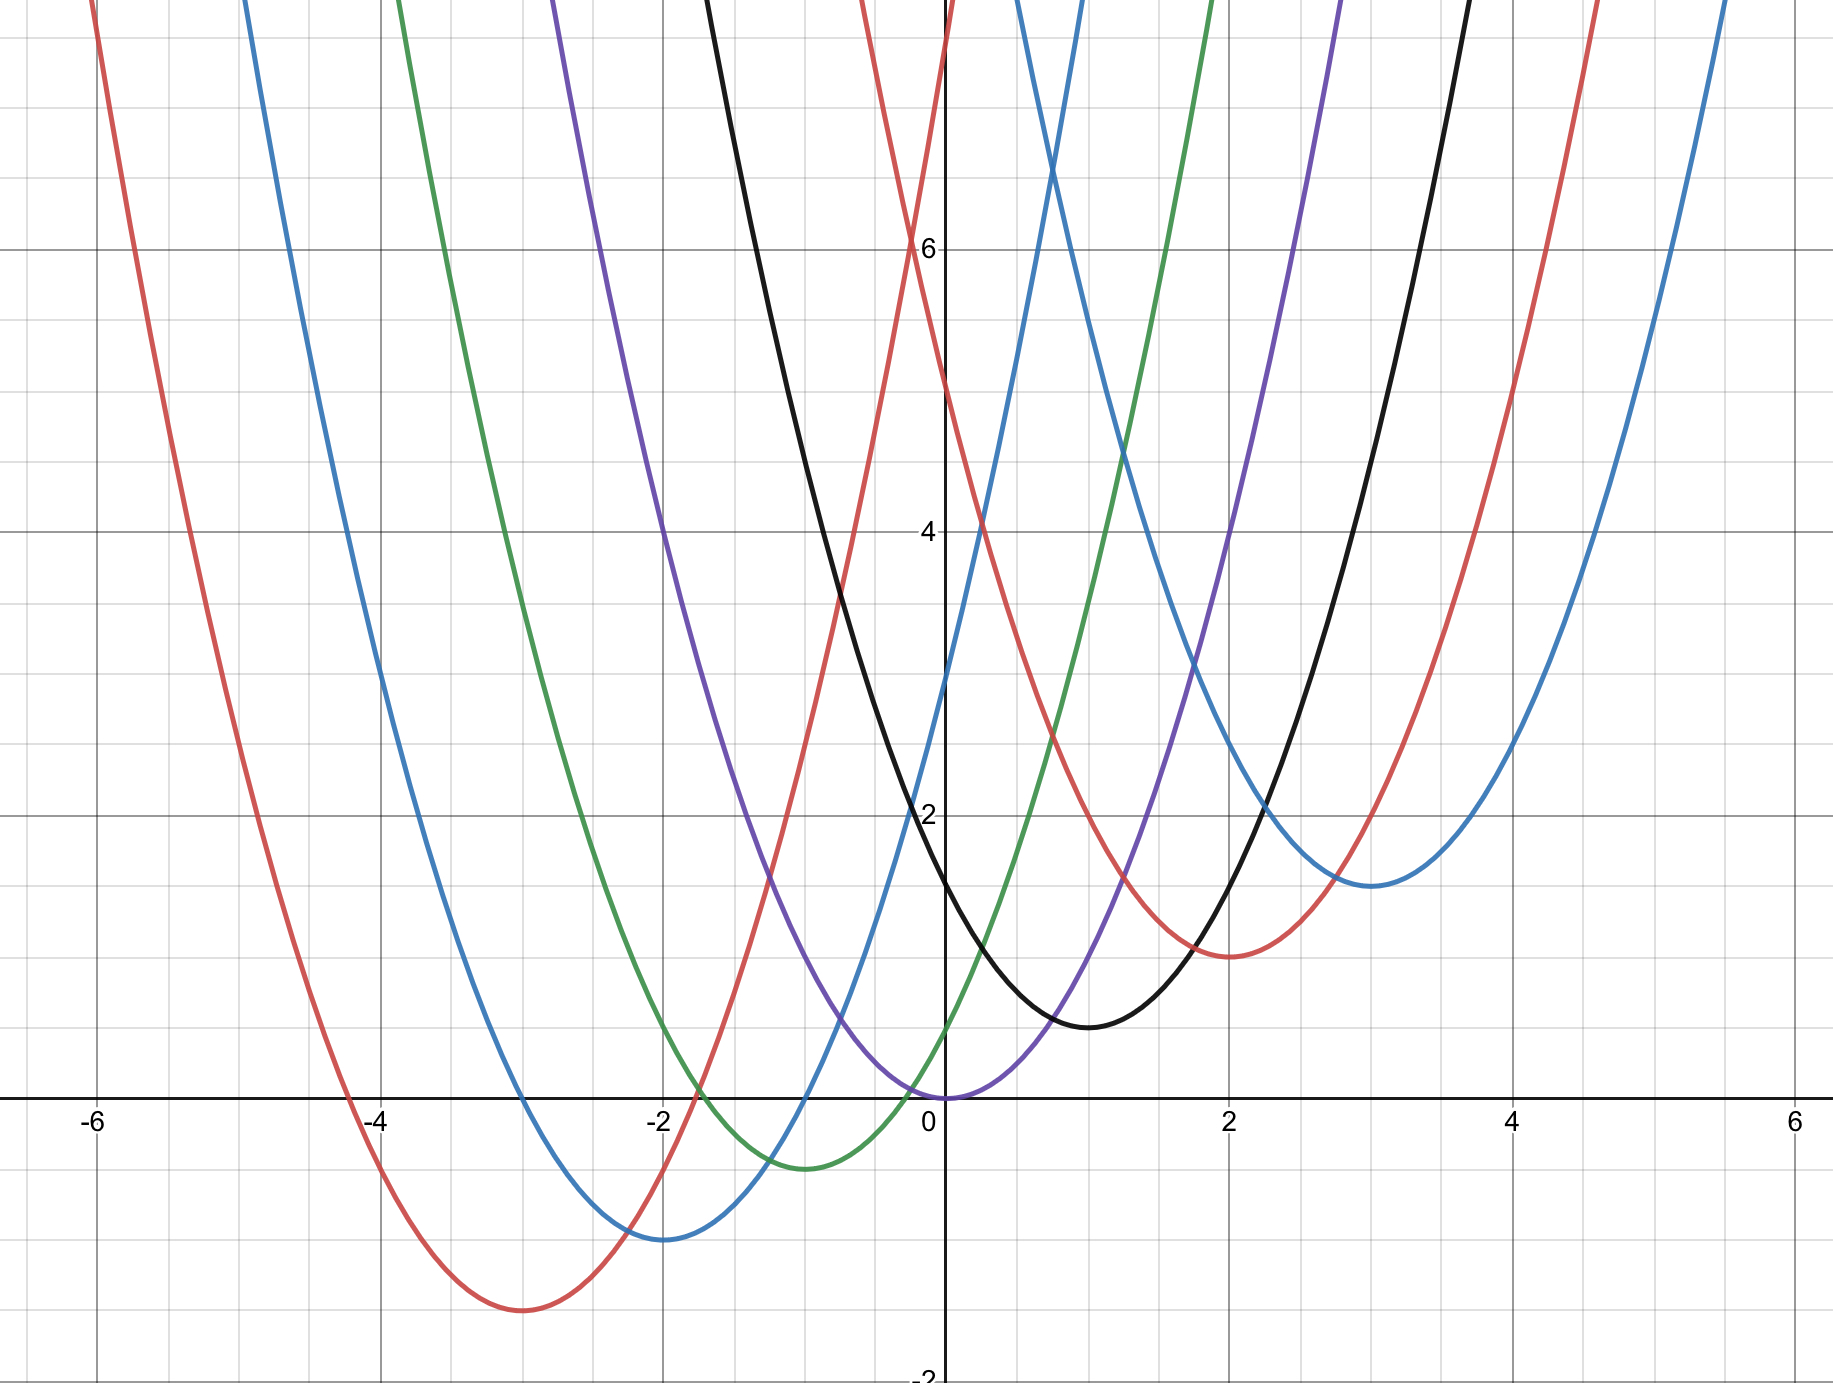
\includegraphics[width=1\textwidth]{./images/IMG_1615.jpg}
    \caption{Skizze der Funktionsschar}
    \label{fig:draw}
\end{figure}


\printbibliography[title={Literaturverzeichnis}]

\end{document}

